\documentclass[11pt,a4paper,english]{article}
\usepackage[english]{babel} % Using babel for hyphenation
\usepackage{lmodern} % Changing the font
\usepackage[utf8]{inputenc}
\usepackage[T1]{fontenc}

%\usepackage[moderate]{savetrees} % [subtle/moderate/extreme] really compact writing
\usepackage{tcolorbox}
\tcbuselibrary{hooks}
\usepackage[parfill]{parskip} % Removes indents
\usepackage{amsmath} % Environment, symbols etc...
\usepackage{amssymb}
\usepackage{float} % Fixing figure locations
\usepackage{multirow} % For nice tables
%\usepackage{wasysym} % Astrological symbols
\usepackage{graphicx} % For pictures etc...
\usepackage{enumitem} % Points/lists
\usepackage{physics} % Typesetting of mathematical physics examples: 
                     % \bra{}, \ket{}, expval{}
\usepackage{url}

\definecolor{red}{RGB}{255,10,10}

% To include code(-snippets) with æøå
\usepackage{listings}
\lstset{
language=c++,
showspaces=false,
showstringspaces=false,
frame=l,
}

\tolerance = 5000 % Bedre tekst
\hbadness = \tolerance
\pretolerance = 2000

\numberwithin{equation}{section}

\newcommand{\conj}[1]{#1^*}
\newcommand{\ve}[1]{\mathbf{#1}} % Vektorer i bold
\let\oldhat\hat
\renewcommand{\hat}[1]{\oldhat{#1}}
\newcommand{\trans}[1]{#1^\top}
\newcommand{\herm}[1]{#1^\dagger}

\newcommand{\Real}{\mathbb{R}}
\newcommand{\bigO}[1]{\mathcal{O}\left( #1 \right)}

\newcommand{\di}{\mathrm{d}}

\newcounter{algcounter}
\renewcommand{\thealgcounter}{\Roman{algcounter}}

\newenvironment{algorithm}{%
\refstepcounter{algcounter}
\begin{tcolorbox}
\centerline{Algorithm \thealgcounter}\vspace{2mm}
}
{\end{tcolorbox}}

\newcommand{\figurewidth}{.85\textwidth}

\title{FYS3150/4150\\Computational Physics\\Project 4}
\author{Candidate numbers ?? and ??}
\date{\today}

\begin{document}
\tcbset{before app=\parfillskip0pt}
\maketitle

\begin{abstract}
This project explores the Ising model applied to spins in two dimensions.
\end{abstract}



\section{Introduction}


\section{Theory}

The energy of a spin system in the Ising model 
\begin{gather}
E = -J\sum_{\expval{kl}}^N s_k s_l
\end{gather}
With $s_i = \pm 1$, N number of spins, J coupling constant, summed over 
the closest neighbours only.

\begin{figure}[H]
\centering
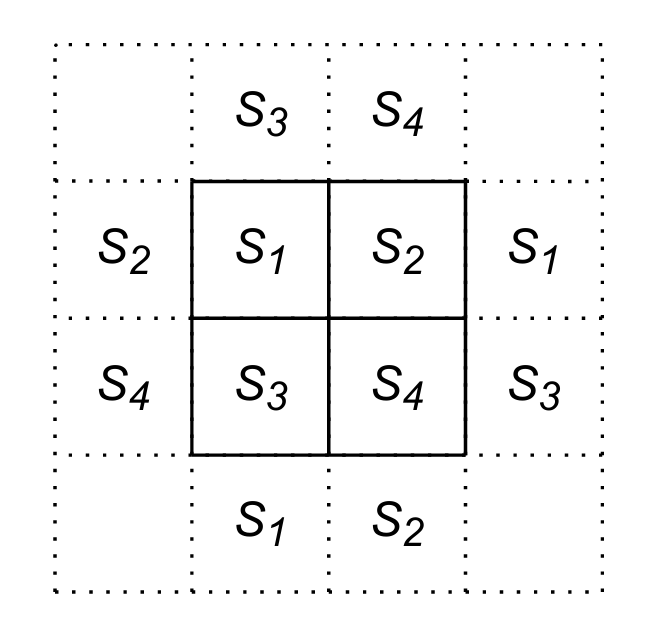
\includegraphics[scale=0.15]{pics/simple_lattice.png}
\caption{ Illustration of the simple, ''$L=2$''-lattice and a graphical interpretation the periodic boundary conditions.}
\label{eq:spin_neighbours}
\end{figure}

Using periodic boundary conditions,
\begin{gather}
s_k = s_{k \pm L}
\end{gather}

For the simple case of only two spins in each dimension($L=2$) the energies are:
\begin{align*}
E_1 = -J\sum_{<1l>}^{N}s_1 s_l = -J[2(s_1 s_2)+2(s_1 s_3)] \\
E_2 = -J\sum_{<2l>}^{N}s_2 s_l = -J[2(s_2 s_1)+2(s_2 s_4)] \\
E_3 = -J\sum_{<3l>}^{N}s_3 s_l = -J[2(s_3 s_1)+2(s_3 s_4)] \\
E_4 = -J\sum_{<4l>}^{N}s_4 s_l = -J[2(s_4 s_2)+2(s_4 s_3)] 
\end{align*}


\subsection{Statistical mechanics}
\begin{gather}
Z = \sum_i \exp(-\beta E_i)
\end{gather}

\section{Implementation}

\subsection{The metropolis algorithm}

\subsubsection{Choice of random number generator}

\subsection{Test environment}

\section{Results}

\subsection{Reproduction of results}

To see benchmark calculations along with programs used see:\\
\url{https://github.com/mulimoen/FYS3150CompPhy/}\\
Under the folder \url{Project 4}.

\section{Conclusion}

\section{Refrences}



\end{document}